\chapter[Código]{Código}
\label{Chap5}

\section{Creación de Spiders}
Una vez instalado Scrapy, en nuestro directorio escogido escribimos el siguiente comando para generar un nuevo proyecto de Scrapy.

\begin{verbatim}
	scrapy startproject miproyecto
\end{verbatim}

Nos creara un nuevo directorio con el siguiente contenido.

\begin{figure} [h!]
	\centering
	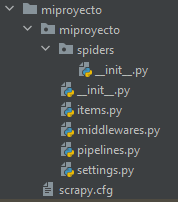
\includegraphics[width=0.3\textwidth]{fig/estructura_proyecto_scrapy.png}
	\caption[Estructura del proyecto recién creado]{Estructura del proyecto recién creado}
	\label{fig:ej11}
\end{figure}

Primero entraremos en el directorio recientemente creado y luego ejecuteremos el comando encargado de crear la Spider.

\begin{verbatim}
	cd miproyecto
	scrapy genspider mispider webausar.com
\end{verbatim}

En caso de no especificar el protocolo usado por la web Scrapy asumirá que usa HTTPS.
\newline
Tras ejecutar el comando la Spider habrá sido generada dentro de la carpeta spiders.

\begin{figure} [h!]
	\centering
	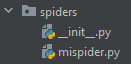
\includegraphics[width=0.3\textwidth]{fig/primera_spider.png}
	\caption[Directorio de almacenamiento de las Spider]{Directorio de almacenamiento de las Spider}
	\label{fig:ej12}
\end{figure}

Una vez abierto el archivo vemos que dispone del siguiente código.

\begin{lstlisting}[language=Python]
	import scrapy
	
	
	class MispiderSpider(scrapy.Spider):
		name = "mispider"
		allowed_domains = ["webausar.com"]
		start_urls = ["https://webausar.com"]
	
	def parse(self, response):
		pass
\end{lstlisting}

Como podemos ver Scrapy usa una programación orientada a objetos, siendo cada Spider una clase representada dentro del proyecto.\newline
Analizando las variables definidas vemos las siguientes, name, nombre por el que debemos referenciar la Spider a la hora de ejecutarla; allowed\_domains, indica que dominios podemos visitar, negando la entrada a cualquier dominio que no este definido en ella, es importante no especificar protocolo, de esta manera funcionara para cualquier web ya sea HTTP como HTTPS que pertenezca a ese dominio, de lo contrario se limitara al protocolo indicado; start\_urls, URL inicial sobre la que se hará la request de petición de datos.\newline
El método parse es aquel al que se envía la respuesta obtenida de la web, para realizar el filtrado de la información, quedándote unicamente con la deseada. Este método es invocado automáticamente por la Spider, sin necesidad real de hacerlo tu manualmente.

\subsection{Proceso de obtención de datos}
Para poder realizar es la extracción de los datos, primero debemos ir a la web deseada e inspeccionar su estructuración. Para ello como ejemplo vamos a usar la web de aemet.\newline

\begin{figure} [H]
	\centering
	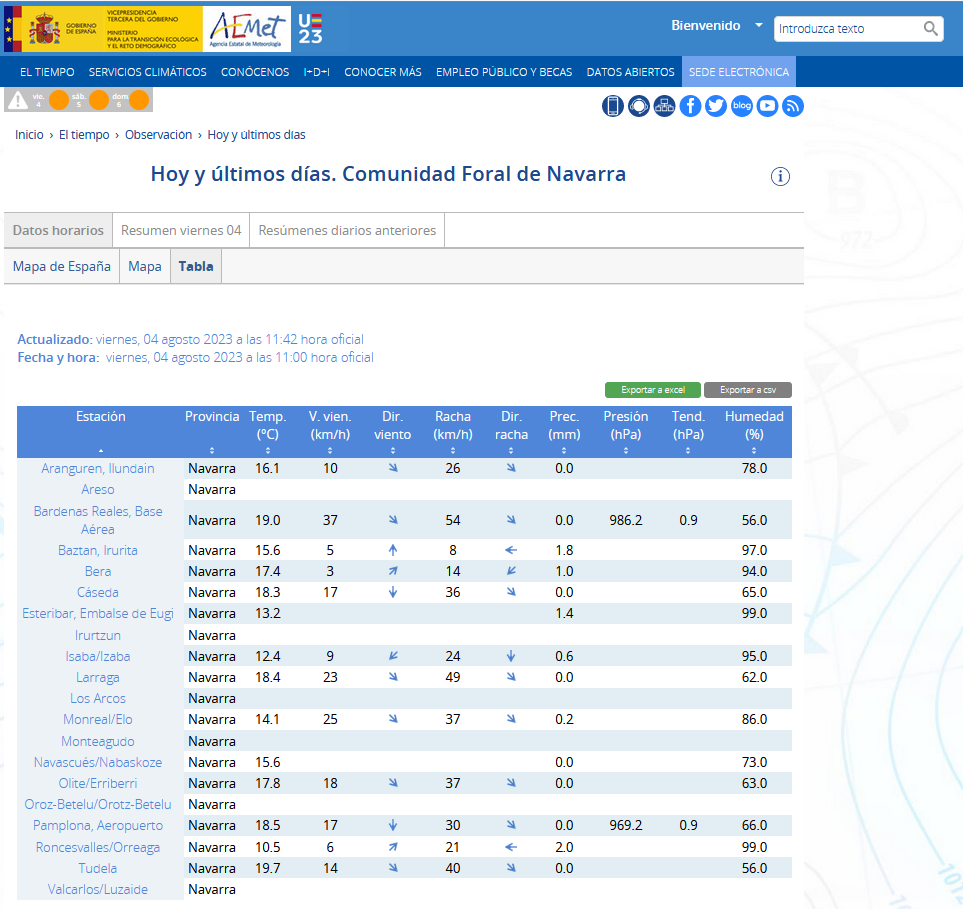
\includegraphics[width=0.8\textwidth]{fig/code_aemet.png}
	\caption[URL de inicio para obtener los códigos de las estaciones de Aemet]{Web de Aemet para obtención de datos}
	\label{fig:ej13}
\end{figure}

Una vez encontrada la web deseada, accediendo mediante el F12 a la herramienta de inspección, buscamos el elemento representativo del dato deseado. En nuestro caso queremos obtener tanto el nombre como el código de la estación. Estos se encuentran ambos en el mismo elemento que forma la primera columna de la tabla.\newline

\begin{figure} [H]
	\centering
	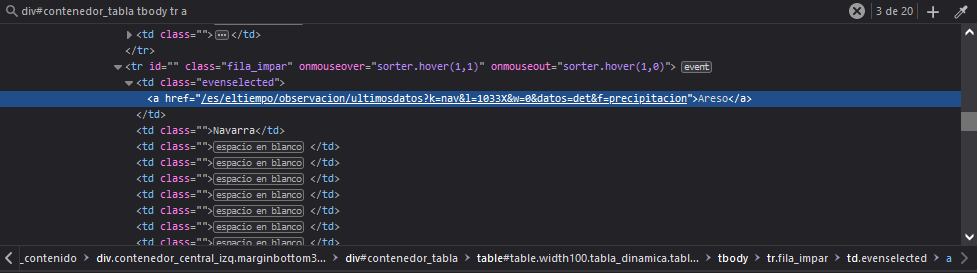
\includegraphics[width=0.9\textwidth]{fig/inspector.png}
	\caption[Inspector de webs de Chrome]{Inspector de webs}
	\label{fig:ej14}
\end{figure}

Por lo que lo primero a lograr es obtener todas las filas de esta. Para ello podemos hacerlo mediante el selector de XPath como el selector de CSS.\newline

\begin{verbatim}
	rows = response.xpath('//div[@id="contenedor_tabla"]/table/tbody/tr')
\end{verbatim}


